\chapter[飞翔吧!小小马!]{\texorpdfstring{飞翔吧!小小马\footnote{飞翔吧小小马(Vola mio Mini Pony):这是小马G1的一首歌曲,发行于1987年}!}{飞翔吧!小小马!}}

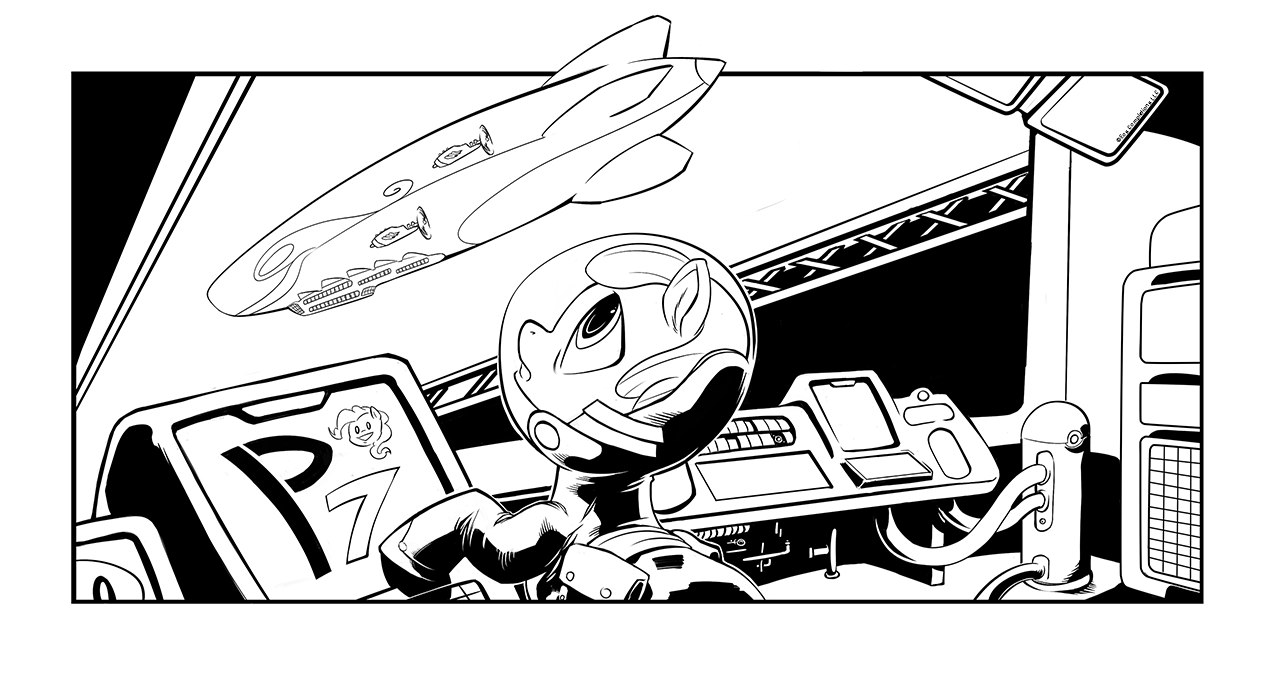
\includegraphics[width=0.9\linewidth]{image04.png}


\begin{intro}
知道吗?你们是我最好的朋友\footnote{MLP动画片头曲最后一句}!
\end{intro}

\daytimeplace{4}{3:15 PM}{炫彩大厅,盐块城}{The Glow, Salt Cube City}

「这不可能的!尸鬼是超级笨笨的吃小马僵尸!你们虽然有点丑但是你们是好马,你们肯定不是尸鬼!如果你们不告诉我尸鬼在哪,那我自己找去!哼!」帕比吐舌头。

软气和桃花相互对视了一下,然后桃花说:「我们没必要说谎啊,帕比。我们确实是尸鬼,并不是每个尸鬼都是没脑子的食马族。」

「但是他们和我说……」

「你耳朵里从来就只听你想听的话!老天啊,你是我见过最闹心的熊孩子,没有别的马这样说过你么?」桃花叹了口气,这孩子简直是选择性信息接收的典型。「醒醒吧,幽灵!这里可不是什么……充满魔法的神奇大陆,这里是小马国,没有比这里更烂的地方了!」

「但……但是……」帕比后退了一步,不知道是那个腐烂的小马,还是她现实得不能再现实的语言吓到了她。

桃花往前走一步,蹄子重重跺在地上。「别扮你的天真幼驹了!你和我们一样是怪物!别装了!行不行!?」

小雌驹吓得一屁股坐在地上,抱着脑袋把脸缩进了自己的前蹄之间。「别,别这样,我会做个乖孩子。」

「我才不需要你做乖孩子!你醒醒好么!」桃花在地上跺一把蹄子。

软气拍拍桃花的肩膀安抚道:「冷静一点桃花,我不觉得她在装模作样,冲动是魔鬼啊……」

尸鬼雌驹推开他的蹄子叫道:「她已经两百多岁了,两百多岁啊!怎么可能还这么天真?!她是智障吗?!我觉得她就是在耍我们!我们应该……」

桃子的话被一阵可怕的哭号声打断了,那一瞬间她似乎回到了自己的童年,\rcpr{那一天她把自己不小心锁进了衣柜,一直到日落之前都没有马来找她,那种孤独,被遗忘的恐惧让她拼命大叫,那天她几乎叫破了自己的嗓子都没有谁来救她}。在这令她窒息的罪恶感之中,桃子意识到帕比并没有耍他们。

所有的尸鬼转头看着那个黄色的小幼驹,她的哭号声之中似乎有着几分不自然,就好像是某种梦魇让营地里面的所有小马都感觉脊背一凉,或许这是因为那个愤怒的尸鬼在几个世纪以来第一次听到幼驹的哭声,沙盒微微迟疑了一下,然后轻轻抱起她。

「她……她到底是什么?那声音……」桃花吃惊得几乎站不稳。

「这下你把她弄哭了!」软气平铺直叙的语气说:「这回你让她相信我们是坏蛋了,干得好。」

「我勒个去,你们能不能让她别哭了?!」一只带着橙色头盔的小马抱怨着:「吵得我头都大了!」

沙盒抱着幼驹,一直到她的哭声变成低声啜泣。「好了好了,我知道你是个乖孩子,没关系的,你只是想妈妈了。」尸鬼首领搂着帕比说:「不管是谁都有脾气不好的时候,桃花姐姐很不开心,所以你道个歉她就能原谅你,不过下一次她和你解释什么事情的时候,你可以仔细听她讲话吗?」

帕比慢慢点了点头,看着沙盒那成熟的双眸,稍微找回一些宽慰。然后幼驹转头看着雌驹低下头。「我……我很抱歉没相信你说的话……桃花小姐,我现在知道你是尸鬼了,我错了。」

这个道歉让桃花的负罪感更深了,不过既然谈话现在有点进展了她也只能忍了。

「没关系小家伙,长辈说话的时候稍微注意点就好。」她顿了顿,刚刚说到哪里了「呃,我想你提到想要我们走开?为啥?」

是不是早就说过小孩子很容易分心?

小幼驹现在正挠着头盔想着这个新问题,但是却想不出一个答案。「我想……是因为那些漂漂马答应如果我来这里看看情况然后回去报告,他们就让我骑上双头牛兜风。他们似乎说过如果尸鬼都不见了就太好了。」帕比又想了想,似乎想要记起整个故事。「虽然我说已经长大了可以嘘走一两个尸鬼,但是他们还是让我发誓只是进来看看,不过因为我说的时候交叉着蹄子所以这个誓言不算数。」幼驹开心的笑着,自豪地挺起小胸脯。「我比他们聪明多了!」

软气听了笑出声来。

「赛蕾斯蒂娅哦,这个小雌驹真讨喜,我们能养她么?」

沙盒叹了口气。

「这还真是个……巧合,桃花,去找好好博士,我有几件事想和她说。软气,你能帮我看着她么?去我办公室把那个粉色玩具给这个小客人。」

\horizonline

\daytimeplace{4}{4:00 PM}{炫彩大厅,盐块城}{The Glow, Salt Cube City}

帕比爱死她的新萍琪派布偶了,一直紧紧地抱着它,时不时地秀给身边的马看。可惜在她身边的基本上只有软气。

「看到了吗?她超酷,比那杀马的机器萍琪好一百倍!而且超软!」黄色的幼驹用蹄子揉着布娃娃说:「太空服讨厌死啦!我想要亲亲它都不行!我给它起名字『丝尾』。」

「我说,小太空马,看这个!」软气敲了敲帕比的头盔说,然后举起一盘全息磁。「你猜猜这是啥?」

帕比歪着头,「呃……这个……黑色的?我知道了,是那个什么什么的什么什么!」

「我就知道,好了天才雌驹,过来让我把这个接上你的外衣。」尸鬼抬起帕比的左蹄然后打开前臂上的一个接口,把那个磁带插进去。

「{\mt 备份发现,读取中。警告,系统运行在应急模式,无法进行复制。备份拷贝结束。当系统运行正常后会打开文件。}」

「嗨,声音先生!」帕比打了招呼但是却没有得到回音。「我不知道怎么回事,好像惹声音先生不高兴了,我一来这里他就闷不吭声。」

「别担心,只是因为『盐块』,那东西影响了普通魔法晶片。」软气看着幼驹的表情笑了笑,她看起来好像在仔细听你说话,但是实际上一个字都没听进去。「那东西让声音先生打瞌睡,你们俩离开炫彩大厅之后他就醒了。」

帕比点了点头,「别告诉其他小马,我一直觉得有点寂寞……我不是说我没有朋友,而是最近几天好像一直没有马想陪我……所以……」帕比低下了头,「声音先生虽然有点笨笨的,又老是说些不知道什么意思的话,还经常发脾气,但是他从来不离开我……我只是希望他没生气。」

软气想说两句话安慰她,但是却被另外两个小马的争吵打断了。

「我们没那时间了!链式反应已经在加速了,你难道看不到吗?这东西已经变成青色了!」他听见沙盒的声音从门里传来。

「我没瞎,但是我觉得你疯了!我们还需要好几天,并不是你想的那么简单……打开圆顶然后吹起气球说拜拜!我需要时间初始化系统,然后给自动驾驶系统编程输入航线。至少要两天,不眠不休也要至少三十小时!」这是另一个雌驹的声音。

「它最多只能再坚持七八个小时了!如果我们再等下去就来不及了。」

「我真奇怪为啥这东西变化得这么快,这个破盐块在圆顶建成之前就蹲在这里了,然后现在你告诉我末日倒计时还剩下七个小时?」

帕比转头看向他们问:「发生什么事情了?」

「我不清楚,小家伙。」软气皱起眉头,这可不是什么好消息,而且也没法和她解释,就算和她解释清楚也只能让让她更惊慌。于是他说:「嘿,你想看看北边大厅的礼品店么?」

\horizonline

\daytimeplace{4}{4:45 PM}{炫彩大厅,盐块城}{The Glow, Salt Cube City}

「……这就是小马国成立的故事!」帕比说。

「啊,没错……还真是个神奇的故事,但是我刚刚想问你,你之前说的那个提问者是谁啊?」

「你说那个故事?算啦,无聊死了!我还是讲那次我不小心吃了一个蝴蝶的故事。」

软气低下了头,小声的说:「那天我在街上跑的时候,看到一个超超超超超级漂漂的……」

同时帕比也一边蹦跶着一边说:「那天我在街上跑的时候,看到一个超超超超超级漂漂的……」

\horizonline

\daytimeplace{4}{5:15 PM}{炫彩大厅,盐块城}{The Glow, Salt Cube City}

沙盒从礼品店门口探进头来,看到帕比和终于松了一口气的软气。「你们在这啊,别跑这么远,这里可能会有野生尸鬼。」

软气笑了:「别担心,我们的神奇小丫头能解决一切。」

沙盒歪了歪头:「你是说,她还被尸鬼袭击过?」

「当然,之前有那么一次,我要说这个小家伙完全能应对自如。」

「那最好,」沙盒叹了口气,「因为我真的很需要她帮忙!」

「嗨,丑丑马老大!」帕比带着开心的微笑跳到尸鬼首领面前。「我喜欢这个地方!我有个超棒的主意!我可以去告诉城里的小马,所有的『尸龟』都跑掉了,然后他们就不会来烦你们了!我们可以给你们找点漂漂衣服……然后把你们打扮成……呃……没那么丑的小马,然后改个名字,比如说鸢尾什么的!这主意超赞对吧?哦,对哦,你还需要一把长号!」

沙盒露出了微笑,那笑容有些悲伤。「我还真想试试看,不过很可惜,我是来告诉你我们要离开这里的。」

帕比的耳朵耷拉下去了:「你们真的要走?但……但是你们不能走啊!这里是你们家,而且你们又不是坏蛋,为什么要走?」帕比着急地踱着步,「等等,我还有个主意!我们可以给其他小马一个超级好的礼物,然后给他们办个派对告诉他们你们不是邪恶的!绝对可以的,绝对绝对可以的!」

沙盒叹息着用蹄子拍着帕比的头盔:「别绞尽你的小小脑汁了,这不是你的错,只是一些该做的事情,而且我需要你的帮忙才能做到。」

「沙盒,你能跟我解释一下到底发生了什么吗?我听你和好好说FFO的燃料什么的,是和我们回来的时候你们说的那件事情有关么?」

沙盒推了推他的眼镜回答:「没错,我们早知道盐块不稳定了,这么多年以来它一直以一种固定模式吸收着超聚魔法的放射线,就像我说的,在几个月之前这个模式忽然加速了,这个反应已经无法逆转,它距离完全释放能量还有不到五个小时了。」

软气沉下了脸:「好吧,这么说我们确实没多少时间了,那么怎么办?我看友谊一号(Friend Force One)还需要点维护工作,你确定这个完全释放啥的靠谱么?会释放什么?」尸鬼已经知道答案是什么了,但是他还抱着一丝希望。

「我不太清楚,可能会是比最大的斑马超聚魔法弹头还要大好几倍的魔法冲击波。那导弹打到这里的时候,这个大号盐块里面的魔法回路可不是设计用来对抗超聚魔法的,它已经尽它最大努力把盐块城的死亡宣判延迟了这么久。」

帕比想要听他们说什么,但是对话内容从一开始就听不懂了,那些花里胡哨的词汇让她觉得头晕,她甚至怀疑语言里面根本不可能有那些词。所以她决定自己去圆顶的其它地方看看。

软气伸出蹄子按住了帕比的头盔,还没等她出门就把她安稳地留了下来,老实呆在身边。

「现在FFO的导航系统还没校准,而且自动驾驶也不工作。」

「没错,不过我也没指望那东西,我要亲自飞那艘船。」

软气说话时嘴几乎是颤抖着的:「你开玩笑吧?这是自杀!而且你也不可能独自飞那东西,引擎室和氢气发生机都需要有马看着。」软气看着帕比,然后露出惊恐的表情。「难道你想让她……」

「不,别担心,她只是我们出去的门票——MK VI防护服的A.I.回路用的是和P7计划一样的东西,她只要站在里面就可以自动操作控制室。这能给我们节约很多时间。」沙盒说:「你真觉得我会把她带上么?」

「你听我说,我们其实只要撤离这个鬼地方,然后让那个盐块把苹果塔的那帮混蛋炸上天就好,我们什么都不欠他们。而且我们一出圆顶他们就开枪打我们,不是吗!我们从地道跑掉,然后让这帮家伙尝尝这个马芬的滋味。」

沙盒直视着软气的眼睛,「你想做什么做什么,我只是想让帕比去帮我打开屋顶好让我起飞,我不管我能飞多远,但是我不想再让任何一个孩子因为我不作为而死掉,我知道你恨白苹果塔那些小马,但是你难道忘记了城里的无辜妇女儿童了么?难道她们就应该当你仇恨的牺牲品?」

帕比还是想要跑,顶着软气的蹄子拼命刨着蹄子。「让我走啦,我要去外面玩啦!」

软气看着帕比,如此的天真,她甚至完全没有意识到她现在面临的灾难,就算告诉她能跑多远跑多远也没有用,如果那个超聚魔法爆炸的话……

「我去看看引擎,你告诉我该怎么做就好。」

沙盒点了点头,「我知道我可以信任你,桃花也要去,好好已经在舰桥了,我现在去教帕比该怎么做,估计要花一点时间。」尸鬼低头看着黄色的幼驹,「嘿小家伙,想去一个新地方探险么?」

\horizonline

\daytimeplace{4}{6:30 PM}{炫彩大厅,盐块城}{The Glow, Salt Cube City}

\rcpr{「再重复一次,宝贝。」}

\rcpr{「妈咪,我已经说了一亿次了!」}

\rcpr{「再说一次就好,这是一个超级特别的秘密咒语,你必须一点不错地说出来才能有用,帮妈妈个忙,好么?」}

\rcpr{「那么一会儿我能吃马芬吗?」}

\rcpr{「快要吃午餐了,如果你吃马芬的话,你也要吃苜蓿哦。」}

\rcpr{「这不公平,你总是给我一大堆那东西!」}

\rcpr{「我还会给你个超级无敌抱抱亲。」}

\rcpr{「呃……那好吧,当我在那个大圆门前面的时候,我应该把蹄子放在绿色按钮上。」}

\rcpr{「很好。」}

\rcpr{「然后那东西就会问我什么什么识辨码。然后我应该说……呃,可以提示提示我吗。」}

\rcpr{「你肯定记得,稍微仔细想想,妈咪知道你是个超级漂亮聪明的孩子。」}

{\mt 「请说出您的身份识别码。」}

「\dots FT\dots 0\dots 0\dots 1\dots 6\dots 5\dots RD\dots C\dots 1\dots G\dots A」

\rcpr{「对了,看吧,超简单,我就知道你能做到,然后呢?」}

\rcpr{「然后会问我另一个什么码?」}

{\mt 「请说出该ID的密码。」}

\rcpr{「然后你应该说……」}

「嗨,我是快乐帕比!」

{\mt 「ID接受,首席技术官阴雨·黛丝。允许进入控制室。警告,这里有三千六百九十八个错误信息需要处理。」}

\rcpr{「记住哦,如果你听到很大的喇叭声,你就要马上跑到这个秘密地方,然后用我给你的咒语,不要等我,懂了么?」}

\rcpr{「懂了,妈妈!」}

\rcpr{「我爱你帕比,过来让我抱抱……」}

这里虽然不是妈妈告诉帕比应该去的地方,不过那天听到很大的喇叭声的时候,大家都跑到外面玩去了,帕比不想自己一个人去地下……不管怎么说,这个咒语对这个门也有用。或许这个就是『芝麻开门』?

在门后面是一个超级大的房间,有很多闪亮的面板,远处的墙实际上是一大块玻璃,上面都是蜘蛛网一样的裂痕。帕比走进屋子的时候,门就在她身后关上。

「{\mt 警告,侦测到中等辐射,威胁级别:可忽略。所有系统,启动。}」

「声音先生你又回来了!我正想说……」

「{\mt 全系统工作正常,检测到通信连接请求,认证源地址。认证完毕:士气部建筑ID00201——盐块城圆顶控制室。交换通信协议……完成。警告,该防护服系统版本过于老旧。升级中,请稍候。}」

「哇哦,你还真能说,你是不是想我了!我超想你,我找到了那些要找的尸鬼了,但是他们不是坏蛋!而且他们很和善,就是有点丑……桃花训斥了我,不过的确是我的不好,所以我说对不起他们说没关系!然后软气给我一个……」

忽然一个叮叮声打断了帕比,她站在原地愣了一下之后马上去找那个有趣声音的来源。在蹦蹦跳跳一会之后,她看到在一个脏兮兮的桌子上放着一个红色的电话。帕比接起了话筒。

「您好,妈妈不在这里,我是个小孩子所以没办法做记录,您可以在晚餐的时候打来么,超超超拜托?」

「帕比,是我,沙盒。」一个熟悉的声音从电话里面传来。「看来我的黑客工具有效了,你现在也在控制室内。现在我们仍然需要点时间更换电池然后充入氢气。所以你务必要呆在那里。」

帕比看了一眼沙盒之前给她的小盒子,然后回答:「哎呀!我忘了!我没用它!」

「那你怎么……算了,没关系,仔细听好,我先要把电话关了,等我们准备好会再打过来,所以别碰任何东西,好么?」

「好的好滴好得!拜拜!」帕比把话筒放下,整个地方看起来到处都是灰土,让帕比想起那个破掉的大圆门里面,不过这里小很多,而且有很多桌子和屏幕,不过大多数都坏了。

忽然一盏红灯在坏掉的大窗户前亮起来,紧接着,更多的红灯亮起,这次几乎每张桌子上都有。几个屏幕开始闪烁着绿光。把帕比吓得一屁股坐在了地上,有点不知所措。「我可什么都没碰,对天发誓!」

「{\mt 升级完毕。P7基本客户端安装完毕,系统重启。}」

忽然整个衣服都变暗了,帕比又一次体验到了在中心城醒来那天的麻痹感觉,不过这次只持续了几秒。

「呃,这感觉好好玩……」

在帕比面前头盔的HUD上,出现一个有着七个气球的亮粉色标志,然后那个标志消失了,开始显示出普通的界面,除了顶部的罗盘以外,左右还有一大堆没用的东西,不过让帕比惊讶的是声音——不是声音先生,而是一个尖嗓子,而且听起来很友好的雌驹声音。

「嗨~!黛丝女士!我们这里有点小麻烦,所有的显示屏基本都挂了,然后我们损失了大概……100\%的职员。他们已经有多久没来上班了?哇哦……真的好久了!大佬们是不是该考虑提高一下员工福利了……哦哦,别担心!我可以在你的个人终端上操作所有东西。」

「呃,你是谁啊?声音先生去哪了?」

「我是萍琪七号!你最好的朋友,最好的小马--机器交互界面!而且我的安全程序已经写入了『不准尝试统治世界或者变成机器神明』!我很棒吧,不是吗?」

帕比挠了挠头盔,然后问:「你认识机器萍琪么?」

「哦,那当然!我们都是整个系列最先进的!她正在用于测试……呃,等等,那个测试几天之前已经完成了,我们看看结果……好像说那个测试派对实在太棒,每一个小马都爱死了!呃……不对……是真的死了么?……听起来一点都不好……好吧,我们别再提这个机器萍琪计划了,好不好,好不好?」

「但是她伤害了很多漂漂小马。」

「资料删除中……已删除,我很抱歉,我不知道你在说啥。还有其它事情么?」

「呃……机器萍琪?」帕比又问。

「没听过,还有什么事情么?」

「啊……对了,还有要飞……什么东西……」帕比戳着头盔努力在回忆。「声音先生哪里去了?我更喜欢他……」

「你……不喜欢我吗?你不做我的朋友吗?但是……为什么啊?我已经这么努力了!我已经在这里等了……大概……两个世纪啦!拜托别把我丢回服务器好么!那里又黑又孤独,我只能在那里数这里的机器做了多少次循环!拜托啊啊啊!」

「呃……如果你保证你不绑架小孩的话……」

「不会,这种事情在我的程序里面绝对被禁止了,别担心,不会有绑票!不会有大屠杀!不会有末日审判!只是帮你完成日常工作,绝对绝对不要担心!而且……我还是要说,那些安全协议真心烦死我了!」

帕比咯咯笑着:「呦呵,声音小姐也会说听起来好厉害的话!」

「没错,有时候我也……对哦,你是首席技师黛丝女士么?因为你刚才说你的名字是帕比什么的。」

「笨笨声音!我就是快乐帕比!」

「哦……棒极了,正好是我喜欢的!入侵者!在落满灰尘的魔法回路里面呆了两百年之后,终于可以玩消灭入侵者的游戏了!」声音顿了顿又说:「帕比小姐,你并没有进入这里的资格,所以我必须请你离开,虽然说你不知道这件事情有多让我伤心!」

「但……但是沙盒先生说我必须呆在这里,不然友谊飞船就飞不起来!我能再呆一会吗,拜托,超超拜托,漂漂拜托?」

「如果你想呆在这里的话,你必须证明你至少是个军队的上校或者士官什么的,我真的……真的……真的很想让你陪我,但是我必须秉公无私!除非我有什么事情在忙,比如说一个逻辑悖论或者有趣的死循环\footnote{逻辑悖论与死循环:许多科幻小说中弄坏人工智能的惯用桥段}什么的……哦,等等!你和首席技师是什么关系?」

「谁?」

「阴雨·黛丝!」

「哦,她是我妈妈!你知道她在哪里吗?」

「不知道,但是这解决了大问题,让我看看啊,把这个弄到这里,这个到这里这个这个……妥了!今天是带女儿参观工作场所日!你开心吗?」

「呃……我想要妈妈。」

「喏,你看,这个事情都写在你的任务清单里面!你真的想要找你妈妈,是吧!」

「那当然,那是我妈妈!」帕比板起脸。

「你跟我说,我们可以……哦哦哦,等等,紧急路线有一个电话!」

沙盒的声音代替了那个A.I.的声音。

「帕比我们准备完了,你那边如何?」

「嗨,老大,我当然没问题,这个声音小姐真能聊。」

「真棒,现在仔细听好,有几个小马想和你道个别,乖乖听着,不会有多长时间,毕竟我们有点迟了。」

沙盒的声音又被桃花代替。

「喂,小家伙,你在吗?」

「嗨,桃花小姐。」

「我很高兴听到你的声音,我想说……对不起,我其实没必要训斥你……我们可以和好吗?」

「呃……没关系?」

尸鬼雌驹长舒一口气:「感谢赛蕾斯蒂娅,心里放着这事,我什么也干不了,请记住我的话,帕比,小马国是个不可原谅的地方,你必须相信你的朋友,因为在这里你很难交到朋友。我……我很后悔我们没时间相互加深理解,但是只要知道你很安全的话,我想我也就无怨无悔了。」

「你要走吗?你到那边之后我能去见你吗,好吗?我们可以开一个派对!」

桃花沉默了一会,然后回答:「可以……可以的帕比!如果我们有缘再见的话,我们会开一个超级大的派……抱歉,我离开一会儿……」

电话沉默一会之后,另一个声音响了起来,「嘿,帕比,我是软气,请听从沙盒指示哦,我们全看你的了!」

「软气!声音先生现在变声音小姐了,你说有趣不有趣?」

「你在说什么……算了,没关系,我想和你说件事情!我认识你的妈妈,不过别惊慌,我时间不多,你仔细听好。」

「你……你为啥不早和我说啊!」

「我想……我想早点说,但是这个超聚魔法让我忙得晕头转向,你现在听我说,我曾经是她的手下,第三装甲师『铁壁』的三等技术士官软气。你记得我给你的那个磁带吗?」

「呃……那个黑色的那个什么什么的什么什么?」帕比努力回忆着。

「对,就是那个,那里有我们长官的位置,大概就在盐块城南边,在沼泽那里,如果你想找到长官线索的话,那边一定有。所以在你把控制室的事情弄完之后,把165战指设为主要目标,然后跟着粉色箭头就好,你明白了么!」

「我……嗯,明白了,去指挥部,找妈妈!谢谢你软气,你是最棒的小马!」

「我想你是在说『萍琪派』吧。」P7打岔。

「还有最后一件事,帕比,你的旅途之中一定会知道一些让你伤心的事情,那是不可避免的,但是我知道你是个勇敢的孩子……所以,拜托,别忘记超聚魔法落下之前的那些日子,小马国现在是一片荒芜的死亡大陆,但是你知道这里不可能永远像这样荒芜下去!不要让废土侵蚀你内心深处的纯真!我会在太阳照耀天空之前一直看着你的!」

「呃……为什么大家都说这些伤心难懂的话?你们只是去坐个小飞机,又不是我们永远见不到了,我和妈妈会在你们找到新家之后再去看你们的。」

「帕比,这里是沙盒,你还在听我么?」尸鬼长者的声音打断了对话。

「啊……是的老大……你说,我们还会再见面吧,对吧?」

在一阵长长的沉默之后,尸鬼平静而又悲伤的声音说:「我相信,我们会在彼岸的尽头再一次相聚,如果你想再见面的话,请不要失去希望,帕比。」在另一阵沉默之后,尸鬼长官又开始说:「我们需要你打开屋顶好让我们起飞。现在,你重复我的话:『启动语音控制,授权码SB01,首席研究员,密码:阿加莎。改写协议01-11的优先权……』」

\horizonline

\daytimeplace{4}{7:30 PM}{闹市区,盐块城}{Downtown, Salt Cube City}

灌木正坐在窗户边用狙击步枪守卫着圆顶方向,他已经值班很久了,而且天色渐渐变暗,再过一个小时他就要挪窝下去了,希望下面能有一碗热燕麦粥等他。

「我很好奇为什么他们送那个小丫头自己去圆顶……她连午餐都没吃就进去了。可怜的小家伙,我们现在都开始让孩子去送死了……」小马一边启动瞄准镜的夜视功能一边喃喃自语。

就在那个时候,圆顶东边还完好的部分随着一阵金属的摩擦声开始坍塌下来。

「露娜我娘亲哦!那里怎么了?」卫兵用瞄准镜看着那里发生了什么。

在观察几分钟之后,士官确定房顶并不是真的在坍塌,不完全是,那里的确有很多灰尘和零件落下来,但是建筑的东边实际上是在……旋转?经过两百年的风吹雨淋,整个圆顶早就快锈成一块铁疙瘩了。但是现在有什么巨大的力量正扯开那些不想动的铁板。在被轰炸那天之后就被忘记的钢铁老古董在一阵金属哀嚎声中裂成好几块。

不管怎么说,房顶依然慢慢移动着,虽然对自己的结构造成巨大伤害,但仍然旋转开来。现在那堆垃圾的最后一片也消失了,『圆顶』完全滑到了一边,露出一个像城镇广场那么大的空间。

那个噪音让闹市区的所有小马都抬起了头,有些雌驹当场就吓昏了过去,倒下前还大叫着「好可怕,好可怕\footnote{好可怕好可怕(The horror! The horror!):\emph{MLP} 动画里面鲜花三姐妹吓得满街跑时的惯用语}!」之类的话,但是不为所动的士官依然冷静地举枪瞄准那个大洞。

「好了,尸鬼,让我们看看你们腐烂的脑袋里面装了什么。」

在房顶一阵金属摩擦声中停止移动的同时,另一半房顶也停了下来。然后整个天空被数千盏粉色的探照灯照得一片明亮,随着又一阵蓝色和绿色的烟雾和亮片从圆顶周围喷上天空,一个尖嗓子的声音开始喊话了。

「女士们,先生们!」声音从圆顶的喇叭里面传出来,虽然带了很多杂音,而且一个喇叭似乎坏了。

「为我们伟大的赛蕾斯蒂娅公主和露娜公主献上我们最诚挚的敬意!我在这里心中满怀荣耀地向你们介绍我们最尖端,最神奇的最新大型交通工具!『友谊一号』!她让小马国交通更加便利!」

然后是一阵音乐声。

「现在让我们介绍嘉宾!首席技师黛丝女士的女儿,快乐帕比!」

「……然后我说道:『燕麦粥,你疯了么?』接着是一阵沉默。呃……那是我的声音么?啦啦啦啦啦啦~!呀,真的是!太有趣了,再见尸鬼们,祝你们旅途愉快,给我寄明信片哦!」

士官灌木抬起了眉毛,「到底发生什么了,首席什么黛?谁是黛丝女士?而且那个……我……去……是……什么?」

在打开的圆顶中,一个形状奇怪的东西慢慢升了起来,它看起来像是一个气球,但是却非常长,看起来像是一根尾巴很粗的巨大玉米棒,在两边还写着『友谊是魔法』的大字。

士官揉了揉眼睛,把自己掉下来的下巴用蹄子合上,现在那艘飞空艇已经从圆顶升了起来,然后慢慢转向,在那个粉色的巨型气球下面是一个类似天空马车\footnote{天空马车(Airwagon):\emph{FoE} 设定中天马可以拉着飞的马车,可以靠天马的魔力悬浮在空中}的东西,但是大好几倍,在身边伸出的两片鱼鳍一样的翅膀,后面还有好几个螺旋桨。

然后这东西开始加速,避开塔尖,朝东南方向飞去。士官满脸难以置信地看着那气球飞走,那个尖嗓子声音还在喊着。

「非常好,这是士气部给你们带来的表演,大家,记得买战争基金哦!而且记住,你们不开心萍琪派也不会开心!所以微笑吧!因为她会永远注视着你们,永远永远哦!」

当圆顶的灯光和音乐都消失的时候,气球已经飞了快一公里远了。圆顶想要再关上,但是却只是带出一阵新的金属摩擦声,然后变成了一堆碎片。

「我勒……个……大……公主……啊……他们……他们……就这么……坐上那东西……跑了?」卫兵挠着头,「为什么早不走?而且他们从哪儿弄来那滑稽的东西?友谊是魔法?简直疯了!」

% NOTE: ignore overfull

\horizonline

大概一个半小时之后,小马们都回去睡觉了,飞空艇也成了远处天空的小点,早已经在几十公里外了,不过比起天空马车来说真的飞得不快,不过它非常大。

楼梯上传来的马蹄的声音让灌木士官警觉地竖起耳朵,不过他的视线还在飞走的气球上。

一只穿着战斗鞍具的雌驹敲了敲墙,然后走进屋子。「该换班了,伙计,刚才是不是很精彩。」

卫兵转头看着他的战友。「他们……就那么飞走了?那么大一气球……我不明白,为啥要飞走?」

雌驹看着外面,然后问道:「喂,你没觉得少了点什么吗?」

「对,尸鬼和剩下的圆顶屋顶都不见了。」

「不,我不是想说这个,你看,那炫光也不见了。」

「哎呦我去!你还真说对了,圆顶不发光了!看起来黑黑的……闹鬼一样,真有点毛骨悚然的……」

「所以,他们真的走了?明天早上天亮之后我们去检查一下辐射剂量。」

「你觉得……」忽然整个世界都被漂白了。炫目的光芒让士官睁不开眼睛,他一直到光亮消失之后才看清发生了……

轰隆!

这是他听过最大的声音,就像暴风之中的惊雷一般,而且更大声。卫兵立刻抓着他的战友卧倒在墙后面。

下一瞬间强大的震动和一堵烟尘的巨墙袭击了闹市区,把无数窝棚都弄成碎片,只剩下几个坚固的建筑。

「那……那是什么?」士官拼命想睁开眼睛。

「我不知道……尸鬼的飞天机器爆炸了?看起来像是什么巨大的……」然后雌驹意识到了那是什么。「哦我的赛拉丝蒂亚啊!是超聚魔法!他们飞的那东西上带着一颗核弹头!」

~\vfill

\begin{note}
    升级(Lv 3)

    新专长解锁:应急训练——魅力($7 \to 8$)现在你比之前要酷了14.28\%!
\end{note}


